% GNUPLOT: LaTeX picture with Postscript
\begingroup
  \makeatletter
  \providecommand\color[2][]{%
    \GenericError{(gnuplot) \space\space\space\@spaces}{%
      Package color not loaded in conjunction with
      terminal option `colourtext'%
    }{See the gnuplot documentation for explanation.%
    }{Either use 'blacktext' in gnuplot or load the package
      color.sty in LaTeX.}%
    \renewcommand\color[2][]{}%
  }%
  \providecommand\includegraphics[2][]{%
    \GenericError{(gnuplot) \space\space\space\@spaces}{%
      Package graphicx or graphics not loaded%
    }{See the gnuplot documentation for explanation.%
    }{The gnuplot epslatex terminal needs graphicx.sty or graphics.sty.}%
    \renewcommand\includegraphics[2][]{}%
  }%
  \providecommand\rotatebox[2]{#2}%
  \@ifundefined{ifGPcolor}{%
    \newif\ifGPcolor
    \GPcolortrue
  }{}%
  \@ifundefined{ifGPblacktext}{%
    \newif\ifGPblacktext
    \GPblacktexttrue
  }{}%
  % define a \g@addto@macro without @ in the name:
  \let\gplgaddtomacro\g@addto@macro
  % define empty templates for all commands taking text:
  \gdef\gplbacktext{}%
  \gdef\gplfronttext{}%
  \makeatother
  \ifGPblacktext
    % no textcolor at all
    \def\colorrgb#1{}%
    \def\colorgray#1{}%
  \else
    % gray or color?
    \ifGPcolor
      \def\colorrgb#1{\color[rgb]{#1}}%
      \def\colorgray#1{\color[gray]{#1}}%
      \expandafter\def\csname LTw\endcsname{\color{white}}%
      \expandafter\def\csname LTb\endcsname{\color{black}}%
      \expandafter\def\csname LTa\endcsname{\color{black}}%
      \expandafter\def\csname LT0\endcsname{\color[rgb]{1,0,0}}%
      \expandafter\def\csname LT1\endcsname{\color[rgb]{0,1,0}}%
      \expandafter\def\csname LT2\endcsname{\color[rgb]{0,0,1}}%
      \expandafter\def\csname LT3\endcsname{\color[rgb]{1,0,1}}%
      \expandafter\def\csname LT4\endcsname{\color[rgb]{0,1,1}}%
      \expandafter\def\csname LT5\endcsname{\color[rgb]{1,1,0}}%
      \expandafter\def\csname LT6\endcsname{\color[rgb]{0,0,0}}%
      \expandafter\def\csname LT7\endcsname{\color[rgb]{1,0.3,0}}%
      \expandafter\def\csname LT8\endcsname{\color[rgb]{0.5,0.5,0.5}}%
    \else
      % gray
      \def\colorrgb#1{\color{black}}%
      \def\colorgray#1{\color[gray]{#1}}%
      \expandafter\def\csname LTw\endcsname{\color{white}}%
      \expandafter\def\csname LTb\endcsname{\color{black}}%
      \expandafter\def\csname LTa\endcsname{\color{black}}%
      \expandafter\def\csname LT0\endcsname{\color{black}}%
      \expandafter\def\csname LT1\endcsname{\color{black}}%
      \expandafter\def\csname LT2\endcsname{\color{black}}%
      \expandafter\def\csname LT3\endcsname{\color{black}}%
      \expandafter\def\csname LT4\endcsname{\color{black}}%
      \expandafter\def\csname LT5\endcsname{\color{black}}%
      \expandafter\def\csname LT6\endcsname{\color{black}}%
      \expandafter\def\csname LT7\endcsname{\color{black}}%
      \expandafter\def\csname LT8\endcsname{\color{black}}%
    \fi
  \fi
    \setlength{\unitlength}{0.0500bp}%
    \ifx\gptboxheight\undefined%
      \newlength{\gptboxheight}%
      \newlength{\gptboxwidth}%
      \newsavebox{\gptboxtext}%
    \fi%
    \setlength{\fboxrule}{0.5pt}%
    \setlength{\fboxsep}{1pt}%
\begin{picture}(9360.00,5040.00)%
      \csname LTb\endcsname%%
      \put(4680,4854){\makebox(0,0){\strut{}Coefficients for transmitted wavepacket}}%
    \gplgaddtomacro\gplbacktext{%
      \colorrgb{0.50,0.50,0.50}%%
      \put(834,504){\makebox(0,0)[r]{\strut{}$0$}}%
      \colorrgb{0.50,0.50,0.50}%%
      \put(834,907){\makebox(0,0)[r]{\strut{}$0.1$}}%
      \colorrgb{0.50,0.50,0.50}%%
      \put(834,1310){\makebox(0,0)[r]{\strut{}$0.2$}}%
      \colorrgb{0.50,0.50,0.50}%%
      \put(834,1713){\makebox(0,0)[r]{\strut{}$0.3$}}%
      \colorrgb{0.50,0.50,0.50}%%
      \put(834,2116){\makebox(0,0)[r]{\strut{}$0.4$}}%
      \colorrgb{0.50,0.50,0.50}%%
      \put(834,2520){\makebox(0,0)[r]{\strut{}$0.5$}}%
      \colorrgb{0.50,0.50,0.50}%%
      \put(834,2923){\makebox(0,0)[r]{\strut{}$0.6$}}%
      \colorrgb{0.50,0.50,0.50}%%
      \put(834,3326){\makebox(0,0)[r]{\strut{}$0.7$}}%
      \colorrgb{0.50,0.50,0.50}%%
      \put(834,3729){\makebox(0,0)[r]{\strut{}$0.8$}}%
      \colorrgb{0.50,0.50,0.50}%%
      \put(834,4132){\makebox(0,0)[r]{\strut{}$0.9$}}%
      \colorrgb{0.50,0.50,0.50}%%
      \put(834,4535){\makebox(0,0)[r]{\strut{}$1$}}%
      \colorrgb{0.50,0.50,0.50}%%
      \put(936,318){\makebox(0,0){\strut{}$0$}}%
      \colorrgb{0.50,0.50,0.50}%%
      \put(1657,318){\makebox(0,0){\strut{}$1$}}%
      \colorrgb{0.50,0.50,0.50}%%
      \put(2377,318){\makebox(0,0){\strut{}$2$}}%
      \colorrgb{0.50,0.50,0.50}%%
      \put(3098,318){\makebox(0,0){\strut{}$3$}}%
      \colorrgb{0.50,0.50,0.50}%%
      \put(3818,318){\makebox(0,0){\strut{}$4$}}%
      \colorrgb{0.50,0.50,0.50}%%
      \put(4539,318){\makebox(0,0){\strut{}$5$}}%
    }%
    \gplgaddtomacro\gplfronttext{%
      \csname LTb\endcsname%%
      \put(342,2519){\rotatebox{-270}{\makebox(0,0){\strut{}$|c_l|$}}}%
      \csname LTb\endcsname%%
      \put(2737,39){\makebox(0,0){\strut{}$l$}}%
      \csname LTb\endcsname%%
      \put(3751,4321){\makebox(0,0)[r]{\strut{}$p_1^\prime = p$}}%
      \csname LTb\endcsname%%
      \put(3751,4042){\makebox(0,0)[r]{\strut{}$p_1^\prime = \langle \xi \hat{\psi}, \hat{\psi}\rangle$}}%
      \csname LTb\endcsname%%
      \put(3751,3763){\makebox(0,0)[r]{\strut{}$p_1^\prime = p_1 + \sqrt{p_1^2 + 4\delta}$}}%
    }%
    \gplgaddtomacro\gplbacktext{%
      \colorrgb{0.50,0.50,0.50}%%
      \put(4718,504){\makebox(0,0)[r]{\strut{}}}%
      \colorrgb{0.50,0.50,0.50}%%
      \put(4718,907){\makebox(0,0)[r]{\strut{}}}%
      \colorrgb{0.50,0.50,0.50}%%
      \put(4718,1310){\makebox(0,0)[r]{\strut{}}}%
      \colorrgb{0.50,0.50,0.50}%%
      \put(4718,1713){\makebox(0,0)[r]{\strut{}}}%
      \colorrgb{0.50,0.50,0.50}%%
      \put(4718,2116){\makebox(0,0)[r]{\strut{}}}%
      \colorrgb{0.50,0.50,0.50}%%
      \put(4718,2520){\makebox(0,0)[r]{\strut{}}}%
      \colorrgb{0.50,0.50,0.50}%%
      \put(4718,2923){\makebox(0,0)[r]{\strut{}}}%
      \colorrgb{0.50,0.50,0.50}%%
      \put(4718,3326){\makebox(0,0)[r]{\strut{}}}%
      \colorrgb{0.50,0.50,0.50}%%
      \put(4718,3729){\makebox(0,0)[r]{\strut{}}}%
      \colorrgb{0.50,0.50,0.50}%%
      \put(4718,4132){\makebox(0,0)[r]{\strut{}}}%
      \colorrgb{0.50,0.50,0.50}%%
      \put(4718,4535){\makebox(0,0)[r]{\strut{}}}%
      \colorrgb{0.50,0.50,0.50}%%
      \put(4820,318){\makebox(0,0){\strut{}$0$}}%
      \colorrgb{0.50,0.50,0.50}%%
      \put(5541,318){\makebox(0,0){\strut{}$1$}}%
      \colorrgb{0.50,0.50,0.50}%%
      \put(6261,318){\makebox(0,0){\strut{}$2$}}%
      \colorrgb{0.50,0.50,0.50}%%
      \put(6982,318){\makebox(0,0){\strut{}$3$}}%
      \colorrgb{0.50,0.50,0.50}%%
      \put(7702,318){\makebox(0,0){\strut{}$4$}}%
      \colorrgb{0.50,0.50,0.50}%%
      \put(8423,318){\makebox(0,0){\strut{}$5$}}%
    }%
    \gplgaddtomacro\gplfronttext{%
      \csname LTb\endcsname%%
      \put(4532,2519){\rotatebox{-270}{\makebox(0,0){\strut{}$|c_l|$}}}%
      \csname LTb\endcsname%%
      \put(6621,39){\makebox(0,0){\strut{}$l$}}%
      \csname LTb\endcsname%%
      \put(7635,4321){\makebox(0,0)[r]{\strut{}$p_1^\prime = p$}}%
      \csname LTb\endcsname%%
      \put(7635,4042){\makebox(0,0)[r]{\strut{}$p_1^\prime = \langle \xi \hat{\psi}, \hat{\psi}\rangle$}}%
      \csname LTb\endcsname%%
      \put(7635,3763){\makebox(0,0)[r]{\strut{}$p_1^\prime = p_1 + \sqrt{p_1^2 + 4\delta}$}}%
    }%
    \gplbacktext
    \put(0,0){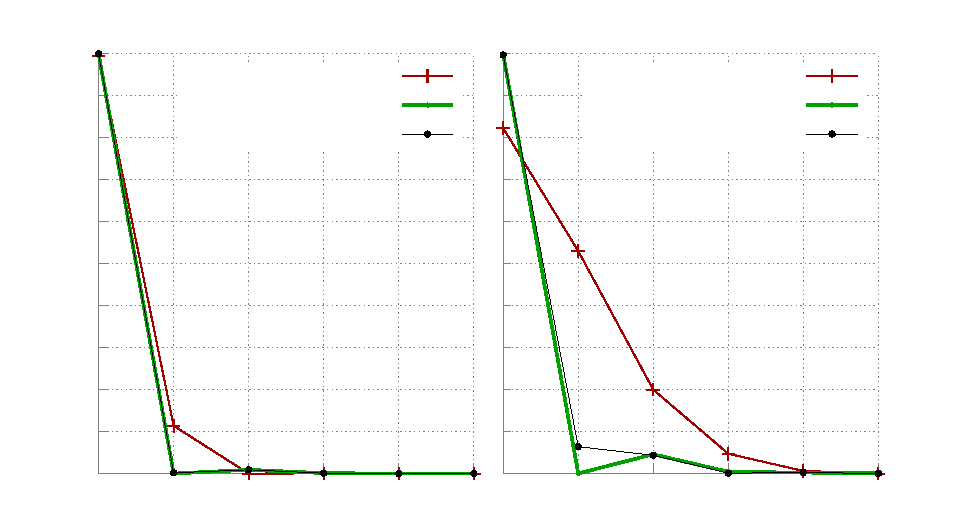
\includegraphics{/home/s1992054/NAQMD/src/Hagedorn/plots/hag_coefficients}}%
    \gplfronttext
  \end{picture}%
\endgroup
